%%%%%%%%%%%%%%%%%%%%%%%%%%%%%%%%%%%%%%%%%%%%%%%%%%%%%%%%%%%%%%%%%%%%%%%%%%%%%%%%
%									HIDING									   %
%%%%%%%%%%%%%%%%%%%%%%%%%%%%%%%%%%%%%%%%%%%%%%%%%%%%%%%%%%%%%%%%%%%%%%%%%%%%%%%%
\subsection{Randomizing the Primitive Code}
\label{sec:hiding}
In \autoref{sec:masking} we have presented a way to protect an implementation by randomizing the encoding of the sensitive data processed through the execution.
Though the latter approach may be theoretically sound, it is practically limited due to the performance overhead incurred by the counter-measure.

An alternative approach consists in designing counter-measures especially sound against a specific type of attacker, not necessarily optimal but most likely to happen in reality.
Therefore, the designed counter-measures, although not theoretically sound, can represent a particularly efficient alternative from a runtime and memory performance point-of-view.
This is the idea behind the development of randomizing the operations processing the intermediate computations.

In a nutshell, without randomized code all the traces follow the same pattern and the sensitive intermediate computations are leaking at the same time coordinates, which makes the use of simple statistical tools particularly relevant for an attacker.
Instead, some randomness in the execution of the elementary operations prevents the attacker from perfectly knowing the expected behavior of the traces, unless adopting specific strategies to mitigate the effects of randomness.
In the following, we review how to implement randomization of the primitive code.

% Different levels of randomization
The implementation of a cryptographic primitive can be described at different levels, from the source code -- if the target is a software device -- to the hardware architecture.
This implies that a developer is provided with a large spectrum of scopes on which randomization may be applied in the operations.

% Software level
At the software or hardware levels, round-based cryptographic primitives -- such as the \gls{aes} -- may be modified in order to incorporate \emph{dummy} rounds.
Inside those rounds, elementary operations may be augmented themselves with dummy operations which are not necessary to proceed the encryption/decryption.
Likewise, for any function looping over independent elementary operations, the latter ones may be executed in a random order.
At a thinner scope, the transcription of the source code into machine code may be randomized thanks to a code polymorphism approach.

% Harware level
Additional scopes of randomization are available at a hardware level.
The use of asynchronous architecture~\cite{renaudin_asynchronous_2000} makes the device prone to a \emph{jitter} effect, causing misalignment in the traces.
Likewise, the use of \emph{dual-rail} logic~\cite{suzuki_security_2006} enables the target device to smoothen the power consumption or the \gls{em} emanations through the execution time, so that it removes the influence of the sensitive intermediate computation.

In the remaining of this section, we further describe some of those approaches which will be investigated in this thesis.
The interested reader can also refer to Chapters 7 and 8 of the \gls{dpa} book by Mangard \etal{}~\cite{mangard_power_2007}.

\paragraph{Shuffling.}
This approach has first been introduced by Herbst \etal{}~\cite{herbst_aes_2006}, and extended by Rivain \etal{}~\cite{rivain_higher-order_2009} and Veyrat-Charvillon \etal{}~\cite{veyrat-charvillon_shuffling_2012}.
% Inspired by DPA book
The idea of shuffling is to benefit from the many elementary functions in the \gls{aes} made of independent (sequences of) operations.
As an example in the \gls{aes}, the \(\ark\) and \(\sub\) process each byte of the state independently from each other.
Likewise, the \(\sr\) and the \(\mc\) process respectively each row and each column independently from each other.
This means that they can be processed in an arbitrary order.
Whereas a naive implementation would process those operations in a trivial order, a protected implementation would leverage the independence in order to process them in a \emph{random} order for each execution of the shuffled algorithm.
This randomness prevents the attacker from perfectly knowing which sensitive variable may be targeted at a given time sample of the acquired trace.
Indeed, the intermediate computation effectively leaking at a given time sample depends on the shuffled indices ordering the independent operations, that have been randomly drawn for this execution.
Those indices cannot be assumed to be known by the attacker, though they can be guessed since the \gls{sca} traces also leak information about them.
Intuitively, the more informative leakage about those indices, the less sound the shuffling counter-measure is.

% Quantitative effect
The effect of shuffling on some attackers can even be quantified.
Indeed, it has been shown that a shuffling over \(t\) different operations had the effect to divide the amplitude of the peaks of \gls{snr} and \gls{cpa} by a factor \(t\)~\cite{clavier_differential_2000,mangard_hardware_2004}, which therefore requires \(t\) times more traces to succeed the attack compared to the same unprotected implementation.
Moreover, Veyrat-Charvillon \etal{} showed an analogous effect of the shuffling on the \gls{mi} between the leakage and the target sensitive variable, when considering an attacker with uni-variate leakage models~\cite{veyrat-charvillon_shuffling_2012}.

\paragraph{Insertion of Dummy Operations.}
Although practically sound against attackers focusing only on a few time samples of the trace, the shuffling counter-measure suffers from an intrinsic limitation, \eg{}, when applied to \gls{aes}: there is not enough independent elementary operations to shuffle to make this approach practically sound against an attacker.
That is why developers also consider adding dummy operations to the execution of the targeted implementation, such as suggested by Coron \etal{} at \textsc{Ches}'09~\cite{coron_random_2009}.
By definition, a dummy operation does not have any effect on the final computation, so it allows to somehow artificially increase the number of independent operations to shuffle.
More precisely, rather than a perfect augmented shuffling, the insertion of dummy operations particularly provokes misalignment (\aka{} \emph{de-synchronization}) which are then propagated along the remaining of the trace, whereas shuffling does not induce this effect.
Therefore, the developer can choose the desired effect on the statistical tools used by some potential attackers -- see \autoref{sec:non_profiled_attacks} and \autoref{sec:PoIs}, to guarantee a security level against them.

Nevertheless, if the dummy operations do not leak in the same way as the sensitive operations, the former ones may be easily distinguished from the latter ones by the attacker, and a re-alignment operation may be proceeded in order to mitigate the effect of the counter-measure.

An example is given in \autoref{fig:dummy_op}, depicting a trace chunk containing a leakage from the access of a \gls{lut} carrying a sensitive information, preceded by the insertion of a random number of \textsf{nop} instructions.
The location of the informative leakage is circled in red.
Since the access to the \gls{lut} and the \textsf{nop} do not span the same pattern in the leakage trace, it is not hard for the attacker to intuitively localize the informative leakage.
Hence, provided that the attacker selects the right method, the attack is not likely to be hardened by this dummy operation insertion.

\begin{figure}
	\centering
	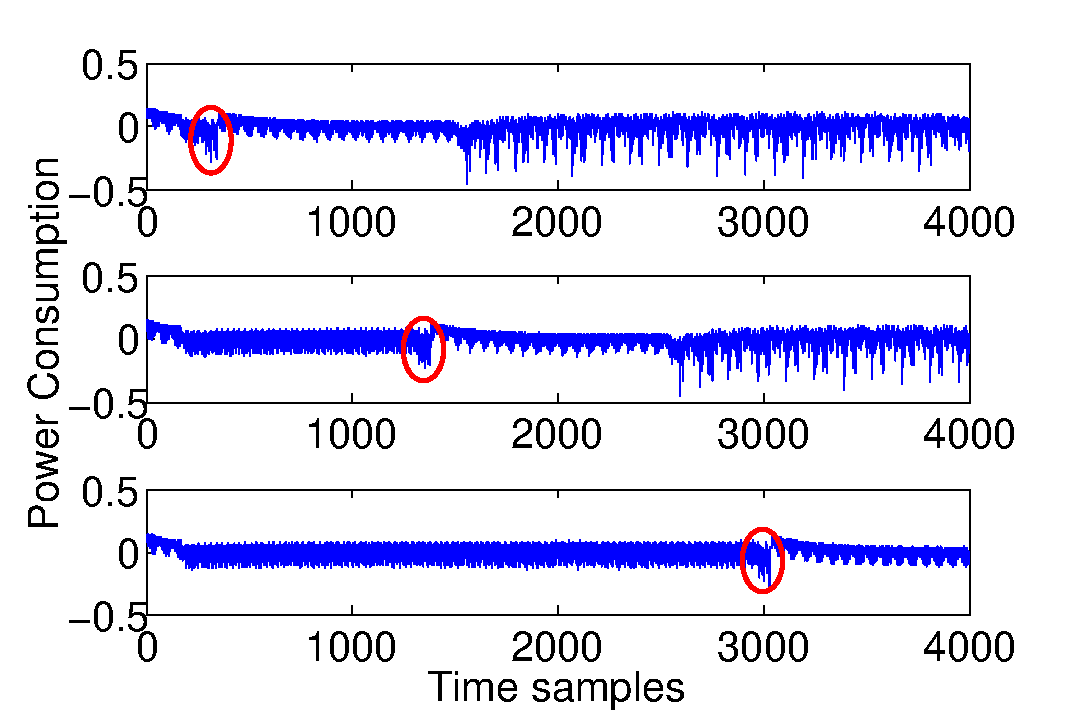
\includegraphics[width=0.5\textwidth]{CW-dataset/CW_shift_traces}
	\caption{An example of dummy operation (\textsf{nop}) randomly inserted before an informative leakage (in red). 
	Courtesy of Cagli \etal{}~\cite{cagli_convolutional_2017}.}
	\label{fig:dummy_op}
\end{figure}

\paragraph{Code Polymorphism.}
Due to the skyrocketing production of \gls{iot}, there is a need for the automated application of protections to improve products’ resistance against \gls{sca} while keeping the performance overhead sufficiently low. 
In this context, some recent works proposed compiler toolchains to automatically apply counter-measures such as bit-slice masking~\cite{belaid_tornado_2020} or a software hiding counter-measure called code polymorphism~\cite{belleville_automated_2019}. 
The working principle of the latter counter-measure relies on the execution of many variants of the machine code of the software device to protect, produced by a runtime code generator. 
The successive execution of many variants aims at producing variable side-channel traces in order to increase the difficulty to realize \gls{sca}. 
One must keep in mind that if code polymorphism is the only counter-measure applied to the target component, information leakage is still present in the side-channel traces. 
Yet, several works have shown the ability of code polymorphism and similar software
mechanisms to be effective in practice against \gls{vertical} \gls{sca}~\cite{agosta_code_2012,courousse_runtime_2016}, \ie{}, up to the point that the leakage characterization techniques presented in \autoref{sec:PoIs}, would not be able to detect information leakage in the traces, and that a \gls{cpa} would require several millions of queries whereas the same attack on the unprotected version of the targeted implementation succeeded within a few hundreds traces~\cite{agosta_meet_2015,belleville_automated_2019}.

We briefly describe the code polymorphism counter-measure applied by the toolchain used by Belleville \etal{}~\cite{belleville_automated_2019}. 
The compiler applies the counter-measure to selected critical parts of an unprotected source code: it inserts, in the target program, machine code generators, called \glspl{sgpc}, which can produce so-called polymorphic instances, \ie{}, many different but functionally-equivalent implementations of the protected components. 
At runtime, \glspl{sgpc} are regularly executed to produce new machine code instances of the polymorphic components. 
Thus, the device will behave differently after each code generation but the results of the computations are not altered. 
The toolchain supports several polymorphic code transformations, which can be selected separately in the toolchain, and most of them offer a set of configuration parameters. 
A developer can then set the level and the nature of polymorphic transformations, hence the amount of behavioral variability.

Hereafter, we detail some code transformations used in this thesis:
\begin{itemize}
	\item \textbf{Register shuffling}: the index of the general purpose callee saved registers are randomly permuted.
	\item \textbf{Instruction shuffling}: the independent instructions are randomly permuted.
	\item \textbf{Semantic variants}: some instructions are randomly replaced by another semantically equivalent (sequence of) instruction(s). 
	For example, variants of arithmetic instructions (e.g. \verb+eor+, \verb+sub+), remain arithmetically equivalent to the original instruction.
	\item \textbf{Noise instructions}: a random number of dummy instructions is added between the useful instructions in order to break the alignment of the leakage in the traces. 
	Noise instructions are interleaved with the useful ones by the instruction shuffling transformation.
\end{itemize}

We emphasize on the fact that the sensitive variables are only manipulated by the polymorphic instances (\ie{}, the generated machine code), and not by the \glspl{sgpc} themselves. 
\glspl{sgpc} are specialized code generators, and their only input is a source of random data (a \gls{prng} internal to the code generation runtime) driving the code generation. 
Hence, \glspl{sgpc} only manipulate instruction and register encodings, and never manipulate secret data. 
Thus, performing an \gls{sca} on side-channel traces of executions of \glspl{sgpc} cannot reveal a secret nor an information leakage. 
However, \glspl{sgpc} manipulate data that are related to the contents of the buffer instances, \ie{}, the structure of the generated code, the nature of the generated machine instructions (useful and noise instructions), \etc{} 
\gls{sca} performed on \gls{sgpc} traces could possibly be helpful to reveal sensitive information about the code used by the polymorphic instances, but to the best of our knowledge, there is no such work in the literature. 
As such, this research question is out of the scope of this thesis.